\chapter{Fundamentação Teórica} \label{cap2}


Este capítulo aborda, de forma sucinta, os fundamentos teóricos que foram aplicados no planejamento e implementaçao deste projeto.



\section{Aprendizado de Máquina}

Aprendizado de máquina(AM) é uma área da inteligência artificial cujo objetivo é o desenvolvimento de técnicas computacionais sobre o aprendizado, bem como a construção de sistemas capazes de adquirir conhecimento de forma automática. Um sistema baseado em aprendizado trabalha por meio de experiências acumuladas e de soluções bem-sucedidas de problemas anteriores  \cite{monard2003}. Normalmente, algoritmos de aprendizado utilizam experiências anteriores, denominadas conjunto de treino, para auxiliar no processo de tomada de decisão.  

Existem três diferentes tipos de aprendizado: supervisionado, não-supervisionado e semi-supervisionado. A diferença entre esses tipos de aprendizado é se o método utiliza ou não utiliza o rótulo de teino. No aprendizado supervisionado, esse rótulo é conhecido, enquanto que no aprendizado não-supervisionado os exemplos não vistos. Já no aprendizado semi-supervisionado, o conjunto de treinamento consiste de uns poucos exemplos rotulados e muitos não rotulados\cite{chappelle2006}. O escopo deste trabalho se encontra no aprendizado supervisionado. 


\subsection{Aprendizado Supervisionado}
O objetivo do aprendizado supervisionado é construir um modelo que consegue fazer predição através de instâncias de uma base de dados rotuladas. Cada instância é representada por um conjunto de características. Na Tabela \ref{table-dataset} é mostrada a estrutura de uma base. Neste exemplo cada vetor $E_i = [x_{i1},...,x_{iM}]$ se refere a classe $y_i$.

A idéia da aprendizagem supervisionada é o conseguir encontrar uma função desconhecida $f$(função conceito) tal que $y=f(\mathbf{x})$, onde o vetor $\mathbf{x}$ são os atributos de uma instância específica. Na prática, a função $f$ deve conseguir prever o valor correto $y_i$ de uma instância $E_i$ não vista. Normalmente, o número de exemplos da base de dados não é suficiente para descrever a função conceito. Nesse caso, o classificador é visto como uma hipótese $h$ que aproxima $f$, ou seja, $h(x)\approx f(x)$ . Caso os valores dos rótulos $y_1,y_2,...,y_N$ sejam numéricos o problema é denominado de \textit{regressão}, caso sejam valores categóricos o problema é denominado de \textit{classificação}. 

\begin{table}[]
	\centering
	\begin{tabular}{c|cccc|c}
		\hline
		& $A_1$ & $A_2$ & \dots & $A_M$  & Classe(Y) \\
		\hline 
		\hline
		$E_1$ & $x_{11}$ & $x_{12}$ & \vdots & $x_{1M}$ & $y_1$ \\
		$E_2$ & $x_{21}$ & $x_{22}$ & \vdots & $x_{2M}$ & $y_2$ \\
		\vdots & \vdots & \vdots &  $\ddots$ & \vdots & \vdots \\
		$E_N$ & $x_{N1}$ & $x_{N2}$ & \vdots & $x_{NM}$ & $y_N$ \\
		\hline
		
		
	\end{tabular}	
	\caption{Representação da base de dados}
	\label{table-dataset}
\end{table}


De maneira geral, a base de dados é dividida em dois conjuntos: conjunto de \textit{treino} e conjunto de \textit{teste}. O conjunto de treinamento é utilizado para ajustar o classificador. Como dito anteriormente, o classificador é uma hipótese da função conceito $f$ ,logo, é fundamental que o conjunto de treinamento tenha uma distribuição o mais semelhante possível do conjunto original.  O conjunto de teste é utilizado para avaliar o modelo construído. Idealmente, esse conjunto não deve ter exemplos em comum com o conjunto de treinamento.

Em alguns casos, pode ser necessário utilizar um conjunto de \textit{validação}, extraído do conjunto de treinamento, para realizar ajustes no modelo construído pelo algoritmo de aprendizado. Logo tem-se três conjuntos: \textit{treino}, \textit{validação} e \textit{teste}. O treino é utilizado para aprendizagem do algoritmo. O modelo é avaliado através do conjunto de validação. É feita uma alteração dos parâmetros do classificador e outro treinamento é realizado. O intuito é melhorar o desempenho do modelo através desses "ajustes". Dessa maneira os exemplos de validação são indiretamente "vistos" durante o processo de aprendizado, o que obriga que esses exemplos sejam diferentes dos exemplos de testes.

\subsection{Normalização e One-Hot Enconding}
Os algoritmos de aprendizagem de máquina aprendem através dos dados. Dados do mundo real apresentam valores que estão em distintas faixas. A fim de evitar que algum atributo predomine sobre outro ou que inclua alguma ponderação indesejada ao induzir um modelo de AM, é comum fazer uma normalização dos valores de cada atributo. Um forma de normalizar os dados é mostrada na Equação \ref{eq-norm}:

\begin{equation}\label{eq-norm}
x_{ij} = \frac{x_{ij} - \overline{x}}{ \sigma_j}
\end{equation}

onde $\overline{x}$ representa a média do atributo e $\sigma_j$ representa o desvio padrão.

Os algoritmos de AM geralmente possuem como entrada e saída valores numéricos, portanto é necessário converter os valores categóricos da base de dados para valores numéricos. A codificação one-hot é um processo que converte rótulos em vetores binários como mostrado na Figura \ref{fig-onehot}. Uma vantagem dessa codificação é que não cria uma "ordem" numérica nos dados. Essa ordem poderia interferir na indução do classificador, podendo dar maior importância para valores maiores, o que não faz sentido para variáveis categóricas.

\begin{figure}[h]
	\centering
	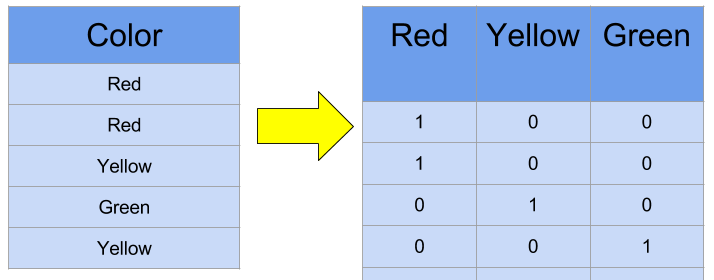
\includegraphics[scale=0.5]{pasta1_figuras/one-hot.png}
	\caption{Codificação One-hot}
	\label{fig-onehot}
\end{figure}

\subsection{K-Nearest Neighbors (KNN)}
Um classificador bastante popular é o K-Nearest Neighbors(K-Vizinhos mais próximos). O KNN utiliza os próprios dados de treinamento como modelo de classificação. Para classificar uma instância de teste, procura-se entre os dados de treinamento os $K$ mais próximos da instância de teste. Por fim, verifica-se qual a classe predominante desses $K$ dados de treinamento, e instância de teste é classificada com essa mesma classe. A cada nova exemplo a ser classificado faz-se uma varredura nos dados de treinamento, o que provoca um grande esforço computacional

O princípio do classificador k-NN é a ``regra dos vizinhos mais próximos''. A hipótese é que, dado um conjunto de exemplos distribuídos sobre o espaço de dados $X$, a ``vizinhança'' de um exemplo $x \in X$ estabelecida por uma função de distância apropriada tende a ser ocupada por exemplos que pertencem à mesma classes que $x$ \cite{hart1967} , como ilustrado na Figura \ref{fig-knn}. Desse modo a informação fornecida pelos exemplos conhecidos que são mais similares a $x$.

\begin{figure}[h]
	\centering
	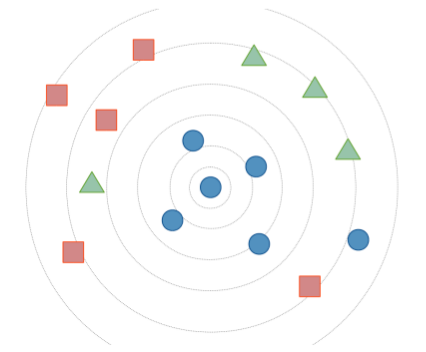
\includegraphics[scale=0.5]{pasta1_figuras/knn.png}
	\caption{Princípio dos k-vizinhos mais próximos}
	\label{fig-knn}
\end{figure}

Para encontrar os vizinhos mais próximos é necessário definir uma medida de similaridade entre dois exemplos. Uma medida de similaridade bastante popular é a \textit{distância euclidiana}. Tal medida calcula a raiz quadrada da norma do vetor diferença entre os vetores $x$ e $y$:
\begin{equation} \label{eq_disteucli}
d(x,y)= \sum_{i=1}^{K} (x_i - y_i)^2
\end{equation}

\section{Redes Neurais Artificiais}
Redes Neurais Artificais são modelos computacionais que buscam simular o processamento de informação pelo cérebro humano. Elas são compostas por unidades simples de processamento, os neurônios, que se unem por meio de conexões sinápticas \cite{zhang1998}. Cada conexão, além de ser altamente especializada, é responsável pelo envio de sinais de um neurônio para outro. Segundo (\textit{Haykin} 2009\cite{haykin2009}) , os neurônios e suas conexões podem ser implementados utilizando-se de componentes eletrônicos ou via simulação programada em computador.

\subsection{Inspiração Biológica e Perceptron}

Um bloco básico de uma rede neural tem algumas semelhanças com um neurônio biológico. O neurônio biológico é uma célula formada por três seçoes com funções específicas e complementares: \textit{corpo},\textit{dentritos} e \textit{axônio}. Os dentritos captam os estímulos recebidos em um determinado período de tempo e os transmitem ao corpo do neurônio, onde são processados. Quando tais estímulos atingirem determinado limite, o corpo da célula envia um novo impulso que se propaga pelo axônio e é transmitido às células vizinhas por meio de sinapses.  Este processo pode se repetir em várias camadas de neurônios. Como resultado, a informação de entrada é processada, podendo levar o cérebro a comandar reações físicas.  \cite{ferneda2006}. A figura \ref{fig-neuronio} ilustra de forma simplificada as partes de um neurônio.

\begin{figure}[h]
	\centering
	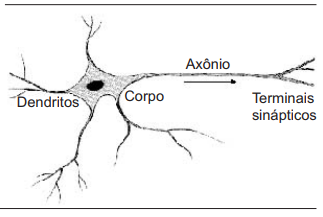
\includegraphics[scale=0.5]{pasta1_figuras/neuronio.png}
	\caption{Representação simplificada de um neurônio}
	\label{fig-neuronio}
\end{figure}

O modelo de um neurônio artifical é apresentado na Figura \ref{fig-guide-1}. Este modelo é composto por três elementos:
\begin{itemize}
	\item Um cojunto de entradas $(x_1,x_2,...,x_n)$ que são multiplicadas por um conjunto e pesos $(p_1,p_2,...,p_n)$;
	\item Um somador $(\sum)$ para acumular o sinais de entrada;
	\item Uma função de ativação que ($\varphi$) limita o intervalo permissível de amplitude do sinal de saída (y) a um valor fixo.
\end{itemize}

\textbf{\begin{figure}[h]
	\centering
	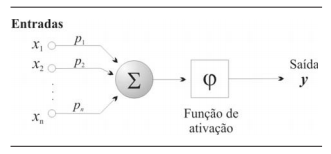
\includegraphics[scale=0.6]{pasta1_figuras/perceptron.png}
	\caption{Modelo matemático de um neurônio}
	\label{fig-perceptron}
\end{figure}}

Esse modelo foi proposto por \textit{McCulloch and Pitts} em 1943 \cite{McCulloch1943} e é conhecido como \textit{perceptron}. A função de ativação ($\varphi$) tem a seguinte definição:
\begin{equation} \label{eq_activation}
\varphi = \left\{ \,
\begin{IEEEeqnarraybox}[][c]{l?s}
\IEEEstrut
1 & if $\sum_{i=1}^{n} p_i x^k_i \geq T$, \\
0 & if $\sum_{i=1}^{n} p_i x^k_i < T$ 
\IEEEstrut
\end{IEEEeqnarraybox}
\right.
\end{equation}
Os valores dos pesos podem ser positivos ou negativos e eles refletem se aquela conexão é inibitória ou excitatória. Um valor positivo ou negativo reflete a importância da respectiva entrada para o processamento. Frequentemente é adicionado um \textit{viés} $b$ na entrada da função de ativação. A forma geral do modelo é descrito como:
\begin{equation} \label{eq-output-percep}
y(k) = \varphi(\sum_{i=1}^{n} p_i(k) x_i(k) +b(k))
\end{equation}
Os pesos sinápticos do Perceptron podem ser adaptados empregando um processo de aprendizado com um número finito de iterações. A aprendizagem é conduzida pela regra de correção de erro conhecida como algoritmo de convergência do Perceptron. Esse algoritmo visa encontrar um vetor de pesos $w$ tal que as duas igualdades da função degrau sejam satisfeitas(\textit{Lippmann}, 1987 \cite{lippman1987})

\subsection{Perceptron multicamadas}

O Perceptron multicamadas(\textit{Multi-Layer Perceptron - MLP}) é uma generalização da rede perceptron. Novas camadas são adicionadas o que possibilita a solução de problemas que não sejam linearmente separáveis. O vetor de entradas \textbf{x} passa pela camada inicial, cujos valores de saída são ligados a camada seguinte. Esse processo se repete até chegar na última camada.(Figura \ref{fig-mlp})  Pode-se arranjar a rede em várias camadas, tornando-a profunda e capaz de aprender relações cada vez mais complexas.

\begin{figure}[h]
	\centering
	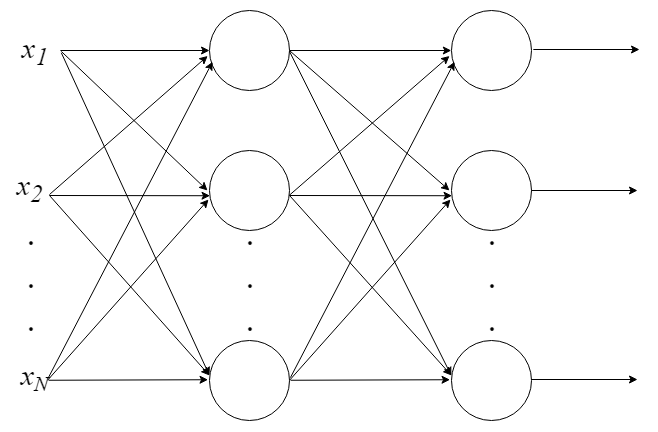
\includegraphics[scale=0.4]{pasta1_figuras/mlp.png}
	\caption{Multilayer Perceptron. Cada círculo representa um neurônio mostrado anteriormente}
	\label{fig-mlp}
\end{figure}

Em 1986, \textit{Rumelhart, Hinton e Williams} \cite{hinton1986} desenvolveram o algoritmo \textit{backpropagation}, que utiliza o gradiente descendente para treinar uma MLP. Este método é composto pelas fases \textit{forward} e \textit{backward}. O objetivo do backpropagation é otimizar os pesos para que a rede neural possa aprender a mapear corretamente as entradas para as saídas. A primeira fase é a ``propragação adiante'' (forward), onde as entradas inseridas na rede se propagam entre as camadas, uma a uma, até a produção das respectivas saídas, portanto a função dessa fase é gerar uma resposta considerando as entradas e os respectivos pesos sinápticos, os quais permanecem inalterados.

Na fase backward é onde a aprendizagem dos pesos é realizada. Esse aprendizado se dá através da otimização (minimização) da função loss, a qual determina a qualidade da classificação do dado de entrada.Essa otimização é realizada através de um método chamado \textit{Gradiente Descendente} que busca a minimização da função \textit{loss} ao alterar os pesos na direção de maior declive do gradiente. O gradiente é calculado na última camada e então é retro-propragado para as camadas intermediárias anteriores que contribuem diretamente para a formação da saída. Cada elemento da camada intermediária recebe é responsável apenas por uma porção do gradiente total. Este processo se repete, camada por camada, até que cada elemento tenha a sua parcela de gradiente para o gradiente total. Baseado no gradiente, é feita uma alteração dos valores dos pesos e bias de modo que a rede aprenda os padrões do conjunto de treinamento.


\subsection{Camada Softmax}

Como explicado em \textit{GoodFellow, Bengio, e Courville}(2016 \cite{Goodfellow2016}), a camada softmax é utilizada como um classificador na camada de saída e tem como objetvio representar a probabilidade de cada classe para cada valor de entrada.

Pela Equação 3.5 nota-se que os valores de saída da camada softmax estão entre 0 e 1, e que a soma de de todas as saídas é igual a 1. Desta forma, cada neurônio de saída representa representa a probabilidade da entrada pertencer a uma determinada classe.

\begin{equation}
softmax(z_i) = \frac{exp(z_i)}{\sum_{j}^{} exp(z_j)}
\end{equation}

\subsection{Função de Perda(Loss Function)}
A função de perda compara a saída da rede para um exemplo de treinamento com o rótulo verdadeiro. Uma função de perda comum é o erro médio quadrático dado pela Equação \ref{eq-eqm}

\begin{equation} \label{eq-eqm}
MSE = 	\frac{ \sum_{i=1}^{N} (y_i - \hat{y_i})^2}{N}
\end{equation}

Quando a saída da rede neural está sendo tratada como uma distribuição de probabilidade é comum utilizar entropria cruzada \textit{cross-entropy}. Ela é usada para quantificar a distâncias entre duas distribuições de probabilidade. Em redes neurais a entropria cruzada comparada a distribuição do que o modelo prediz com a previsão. Ela é definida como:
\begin{equation}
L = - \sum_{i}^{} y_i log(z_i)
\end{equation}
Para problemas de classificação a entropria cruzada é mais adequada.


\subsection{Otimizadores}
A finalidade dos otimizadores é minimizar o valor da função de perda alterando nos pesos da redes. Existem atualmente diversos métodos para alcançar esse fim, esses métodos utilizam de alguns hiperparâmetros para calibrar a forma com que os pesos devem ser atualizados. Dentre os mais utilizados se destacam:
\begin{itemize}
	\item \textbf{ Stochastic Gradient Descent (SGD) com Nesterov Momentum} é um método onde, em uma alusão à mecânica clássica, a velocidade de descida do resultado da função de perda na superfície multidimensional determinada pelo gradiente é calculada e usada para escalar o tamanho do passo que será dado em direção ao ponto mínimo. Utilizando essa velocidade e o valor do gradiente na posição atual é possível prever a próxima posição dessa partícula virtual onde então é calculado o gradiente da nova posição. Os parâmetros são então atualizados baseados nesse segundo gradiente e em um hiperparâmetro denominado taxa de aprendizado (learning rate). \cite{bengio2012}
	\item \textbf{Adagrad} é um método adaptativo de taxa de aprendizado proposto originalmente por \cite{adagrad2011} onde a taxa de aprendizado é normalizada pela raiz da soma dos gradientes de cada parâmetro ao quadrado. Isso tem o efeito de reduzir a taxa de aprendizado dos pesos que recebem gradientes altos e ao mesmo tempo aumentar a taxa de aprendizado de pesos que recebem atualizações infrequentes. Um hiperparâmetro de suavização também é usado para inibir a divisão por zero.
	\item Adam é um método derivado de um outro método chamado RMSprop que basicamente ajusta o método Adagrad para que a taxa de aprendizado não diminua agressivamente. A contribuição do método Adam é adicionar um momento na atualização (semelhante ao Nesterov Momentum) e suavizar os ruídos do gradiente antes de fazer essa operação. Ele herda do RMSprop  adição de uma taxa de decaimento na soma dos gradientes de cada parâmetro que reduz a agressividade de quanto a taxa de aprendizado é reduzida a cada passo. \cite{adam2014}
\end{itemize}

\subsection{Hiperparâmetros de uma Rede Neural}
A maioria dos algoritmos de AM envolvem "hiperparâmetros", que são varíaveis definidas para o algoritmo antes do treinamento com o objetivo de otimizá-lo. Definir os valores de hiperparâmetros pode ser visto como uma seleção de modelos, ou seja, escolher qual modelo usar do conjunto hipotético de modelos possíveis. Em redes neurais os hiperparâmeteros determinam a estrutura da rede (Ex: Número de neurônios em uma camada) ou como a rede será treinada(Ex: Taxa de aprendizado)

\subsubsection{Número de camadas e neurônios em cada camada}
Em problemas de classificação geralmente as redes neurais tem: camada de entrada tem o mesmo número de neurônios do tamanho do vetor de características, camadas escondidas e a camada de saída que tem o mesmo número de classes do problema. Conforme o teorema da aproximação universal \cite{universal1989}, uma rede neural com uma única camada oculta com um número finito de neurônios é capaz de aproximar qualquer função contínua de $\mathbb{R}^n$. Isto quer dizer que teoricamente é possível aproximar qualquer 
\subsubsection{Inicialização dos pesos}
Idealmente, pode ser melhor usar diferentes estratégias de inicialização dos pesos conforme a função de ativação aplicada em cada camada. A distribuição uniforme é comumente utilizada. (*)

\subsubsection{Função de Ativação}
As funções de ativações são usadas para introduzir não-lineariedade nos modelos, que permite que as redes aprendam superfícies de decisões mais complexas. Dentre as funções de ativações mais utilzadas estão a Sigmoid e ReLU(\textit{Rectified Linear Units}). A vantagem  da ReLU é que ela evita o problema de dissipação do gradiente.


\begin{figure}[H]
	\centering
	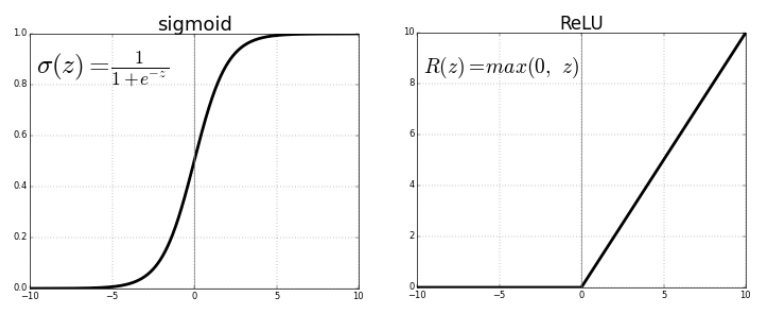
\includegraphics[scale=0.4]{pasta1_figuras/activation_function.png}
	\caption{Softmax vs ReLU. Imagem tirada do site \textit{Towards Data Science} \cite{towardsdatascience}}
	\label{fig-activations}
\end{figure}


\subsubsection{Mini-batches}
O treinamento geralmente é realizado em \textit{batches} também conhecidos como \textit{mini-batches} que são subconjuntos do treino. As razões de utilizar batches e não o treino inteiro são: diminuição do tempo de treinamento; caso o conjunto de treino seja suficientemente grande, uma amostra desse conjunto pode representar de forma \textit{boa} o conjunto original. A tamanho dessa amostra é um hiperparâmetro da rede, sendo geralmente aceito que o treinamento com \textit{batches} maiores resulta numa melhor performance.

\subsubsection{Taxa de aprendizado}

A taxa de aprendizado é um parâmetro constante no intervalo de [0,1] que interfere na convergência do aprendizado. Ela determina o quão ``rápido" as atualizações dos pesos irão em direção do gradiente. Se a taxa de aprendizado for muito pequena, o modelo convergirá muito lentamente; Se a taxa de aprendizado for muito grande, o modelo irá divergir. 

\subsubsection{Número de épocas}
Número de épocas é a quantidade de vezes que o conjunto de treino é passado pela rede. O recomendável é aumentar o número de épocas até que a acurácia do conjunto de validação diminuir, mesmo quando a acurácia do treino aumentar(\textit{overfitting})

\subsection{Regularização}

Além do \textit{tuning} dos hiperparâmetros existe outras maneiras para aumentar a performance da rede e torná-la mais robusta em sua capacidade de generalização. 
Um exemplo é a adição de um termo de regularização na função de perda. Esse termo é introduzido para regularizar os valores dos pesos buscando distribuir melhor o aprendizado por todos os neurônios. A função provavelmente mais usada para este fim é a da regularização L2, onde para cada parâmetro da rede o termo $\frac{1}{2}\lambda \omega^2$ é adicionado ao resultado da função de perda,$\omega$ representando o peso em questão, $\lambda$ sendo a força da regularização e o fator $\frac{1}{2}$ é multiplicado para simplificar o gradiente da função.

Essa regularização penaliza neurônios com pesos muito altos levando a uma distribuição das atualizações para os neurônios com pesos menores. Ao introduzir essa função é necessário lembrar que os pesos também devem ser atualizados pelo gradiente da função de regularização, o que é um passo geralmente realizado após a atualização quanto ao gradiente da função loss.

A introdução da função de regularização ajuda a combater o overfitting e juntamente com ela uma outra técnica que é muito utilizada para esse fim é o \textit{Dropout} \cite{dropout2014}. O Dropout é uma técnica que condiciona à existência de um neurônio na fase de treinamento em função de uma probabilidade predefinida por um hiperparâmetro. Esse método essencialmente desativa neurônios com uma probabilidade p para que a rede seja capaz de otimizar a função loss mesmo sem a presença de todos os seus neurônios.

\begin{figure}[h]
	\centering
	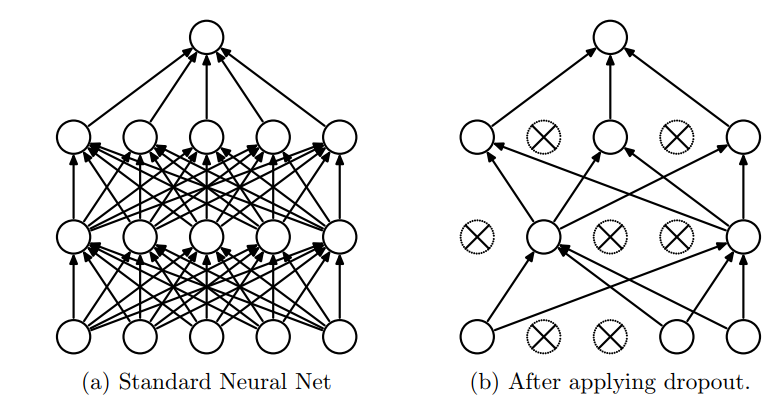
\includegraphics[scale=0.4]{pasta1_figuras/dropout.png}
	\caption{Imagem ilustrando o efeito do Dropout em uma rede neural onde os neurônios marcados foram desativados, forçando a rede nao depender deles, evitando o \textit{overfitting} \cite{dropout2014}.}
	
	\label{fig-dropout}
\end{figure}

\subsection{Redes Convolutivas}

As redes convolutivas  foram desenvolvidas tomando como inspiração o cortéx visual de animais, que contém  agrupamentos de células que detectam luz em pequena escala que são chamadas de campo receptivos. O campo receptivo de um único neurônio sensorial é a região específica da retina em que a presença de um estímulo causa a ativação dele.Os neurônios sensoriais que tem campos receptivos semelhantes se sobrepõe.
Na figura \ref{fig-campo} é mostrada uma representação de um neurônio e o seu campo receptivo. 
\begin{figure}[h]
	\centering
	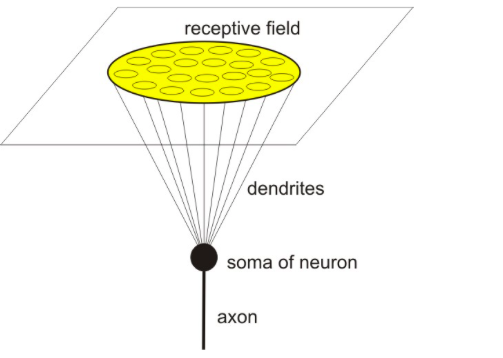
\includegraphics[scale=0.4]{pasta1_figuras/campo_receptivo.png}
	\caption{Campo receptivo de um neurônio. Fonte: \cite{camporeceptivo}}
	
	\label{fig-campo}
\end{figure}

Tais células atuam como filtros locais sobre o espaço de entrada e quanto mais complexa a célula, maior o seu campo receptivo. As redes convolutivas segue esse mesmo princípio de campos receptivos, o que ajuda a diminuir o custo computacional de treinamento. Esse tipo de rede recebe esse nome devido a sua camada mais predominante, a camada de convolução.

Em \cite{haykin2009neural} Haykin divide a estrutura das redes convolutivas em três objetivos principais:

\begin{itemize}
	\item Extração de características: Cada neurônio recebe sinais de entrada de uma determinada janela da camada anterior, possibilitando a extração de características locais. Isto faz com que a posição exata de cada característica (ou pixel, no caso de uma imagem), seja irrelevante, desde que sua posição em relação às características vizinhas seja mantida.
	\item Mapa de características: As camadas são compostas por diversos mapas de características (\textit{feature maps}) que são regiões onde os neurônios compartilham os mesmos pesos. Esses pesos são chamados de filtros ou kernels, e dão robustez ao modelo, fazendo com que ele seja capaz de lidar com variações de distorção, rotação e translação na imagem. O compartilhamento dos pesos também possibilita uma redução drástica no número de parâmetros a serem otimizados.
	\item Subamostragem: Após cada camada de convolução é aplicada uma camada de subamostragem(\textit{subsampling}), que é uma coleta de amostras de cada mapa de característica. Essas amostragens podem ser realizadas através da média, maior ou menor valor das amostras. O que produz uma sumarização do mapa de características
\end{itemize}

A principal aplicação das CNNs é para processamento de informações visuais em particular imagens, pois a convolução permite filtrar as imagens considerando a sua informação visual. Diferente da MLP que vetoriza as imagens a CNN leva em consideração a estrutura espacial entre os pixels vizinhos em uma determinada imagem através da operação de convolução.

A seguir é apresentado os tipos de camadas que geralmente são usadas para redes convolutivas

\subsection{Camada de Convolução}
É na camada de convolução que cada característica específica em alguma posição espacial da entrada é detectada. Os parâmetros dessa camada são distribuídos entre os filtros que tem a mesma ideia dos campos receptivos comentados anteriormente. Os filtros são parâmetros ajustáveis do modelo que devem aprender uma característica específica.  A convolução o ocorre durante a fase \textit{foward}, onde cada um desses filtros são convoluídos com a entrada. Em aprendizagem de máquina os dados são discretos o que acaba simplificando a operação de convolução. O cálculo se torna em um produto entre os elementos de entrada sobrepostos pelos filtros deslocados em toda entrada. 

Alguns hiperparâmetros são importantes na configuração de tal camada\cite{guedes2017}:

\begin{itemize}
	\item Tamanho do campo receptivo(\textit{kernel size}): Para o caso de imagens é o tamanho bidimensional do campo receptivo que será convoluído com a entrada, e pode ter valores como 3x3, 5x5, 16x16. É o mesmo para todos os neurônios da camada. Para o caso em 1-D esse hiperparâmetro  é apenas um inteiro.
	\item Profundidade: É o número de kernels que serão estimulados pela mesma parte do campo receptivo. Cada um desses kernels é responsável por detectar uma característica por toda entrada, constituindo então um conjunto de mapas de características. A Figura \ref{fig-depth} ilustra uma camada de convolução com profundidade cinco.
	
	\begin{figure}[h]
		\centering
		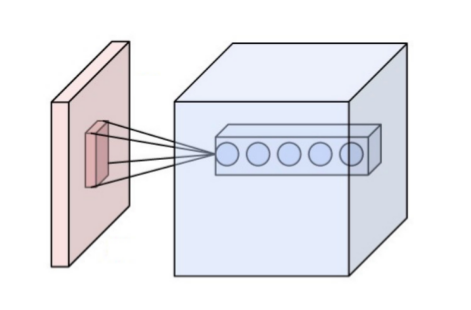
\includegraphics[scale=0.4]{pasta1_figuras/depth_cnn.png}
		\caption{Disposição dos neurônios na camada de convolução e seu campo receptivo. Fonte: \cite{depth}}
		
		\label{fig-depth}
	\end{figure}
	
	\item Stride: É o parâmetro que determina o espaçamento da sobreposição dos campos receptivos. A Figura \ref{fig-stride} mostra que valores diferentes de stride podem alterar o campo receptivo de tais neurônios e o número total dos neurônios de cada fatia da profundidade. Esse parâmetro é decisivo na capacidade de identificar os padrões visuais da entrada, sendo responsável por definir quão refinada será a identificação do padrão mesmo que trasladado, onde o aumento desse refinamento é inversamente proporcional ao desempenho da camada, por conta do maior número de neurônios da mesma.
	
	\begin{figure}[H]
		\centering
		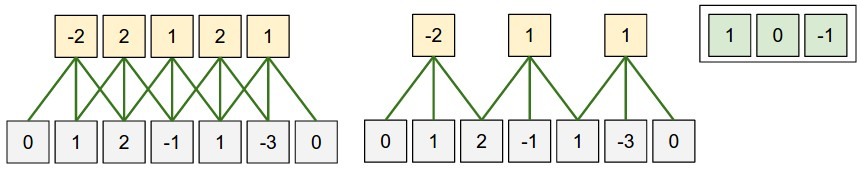
\includegraphics[scale=0.4]{pasta1_figuras/stride.jpeg}
		\caption {Neurônios espaçados por stride 1 e 2 das esquerda para a direita respectivamente. Separados à direita estão os pesos compartilhados entre todos os neurônios. Fonte: \cite{githubstride}}
		\label{fig-stride}
	\end{figure}
	
	\item Zero-padding: Determina qual tamanho do preenchimento com zeros que será adicionado às bordas da entrada. Isso muitas vezes é utilizado para adequar o tamanho da entrada ao stride escolhido, como pode ser visto na Figura \ref{fig-stride} onde o tamanho da entrada (representada unidimensionalmente) é cinco e o zero-padding é um.
\end{itemize}

\subsection{Camada Pooling}
Segundo LeCunn \cite{lecunn2010}, a camada pooling trata cada característica mapeada separadamente, em cada arranjo espacial do mapa de característica chamadas de \textit{pooling} máximo e médio. A figura \ref{fig-pooling} retrata o funcionamento de cada pooling. A entrada é de uma imagem 4x4 e subamostras do pooling de dimensão [2x2]. No caso do pooling médio o valor médio em relação aos quadros em destaque da imagem [4x4] formam cada valor pertinente ao pooling médio, já no pooling máximo, dos quatro valores em destaque, o maior valor representará o valor máximo. 

\begin{figure}[H]
	\centering
	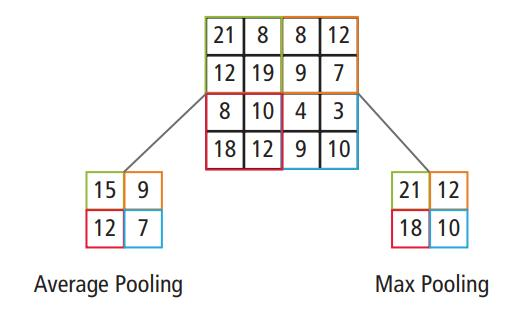
\includegraphics[scale=0.4]{pasta1_figuras/pooling.jpg}
	\caption {Representação de max-pooling e average-pooling Fonte: \cite{githubstride}}
	\label{fig-pooling}
\end{figure}

\section{Séries Temporais}

Série temporal é uma sequência de observações de um fenômeno ao longo do tempo. Geralmente essas medições são feitas em um intervalo de tempo regular. A ordem das amostras é crucial, pois há um dependência entre os dados e uma alteração da ordem pode modificar o significado dos dados. Uma série temporal pode ser definida como:

\begin{equation} \label{eq_TS}
X(t) = (x_1,x_2,...,x_n)
\end{equation}
onde $x_n$ representa uma observação no instante $t$, $n$ o número de observações e $X(t)$ a função que descreve a série temporal em termos de t. Caso a série seja constituída de uma observação em cada instante de tempo ela é chamada de \textit{univariada}. Caso a série foi obtida por uma coleta simultânea de dois ou mais fenômenos ela é chamada de \textit{multivariada}.

As séries temporais estão em diversas áreas do conhecimento como Economia (preços diários dea ações, taxa mensal de desemprego, produção industrial), Medicina (eletrocardiograma, eletroencefalograma), Epidemiologia (número mensal de novos casos de meningite), Meteorologia( precipitação pluviométrica, temperatura diária, velocidade do vento).

\subsection{Aplicações de Séries Temporais}
A análise de séries temporais tem atraído muitos pesquisadores em aprendizado de máquina ao redor do mundo. As principais tarefas envolvendo séries temporais na qual se utiliza aprendizagem de máquina são as seguintes:

\begin{itemize}
	\item \textit{Classificação}: cada série temporal representa uma classe distinta de objetos. Dada uma série temporal, o objetivo é descobrir qual é a classe de objetos ela representa; 
	\item Agrupamento: Dado um conjunto de séries temporais, o objetivo é encontrar uma estrutura natural que permita distribuir as séries em grupos; 
	\item Detecção de Motivos: também conhecido como detecção de \textit{motifs}; o objetivo é encontrar uma ou mais subsequências que aparecem frequentemente na séries;
	\item Detecção de Anomalias: encontrar subsequências ou séries que são inesperadas em algum contexto.
\end{itemize}
Este trabalho está inserido na tarefa de classificações de séries temporais.
\section{Classificação de Séries Temporais}



% Fim Capítulo